\documentclass[preprint,12pt]{elsarticle}

\usepackage{doi}
\usepackage{microtype}
\usepackage{amssymb}
\usepackage{amsmath}
\usepackage{enumitem}
\usepackage{float}
\usepackage{multirow}
\usepackage{booktabs}
\usepackage{siunitx}

\biboptions{sort&compress}
\bibliographystyle{elsarticle-num}


\journal{Journal of \LaTeX\ template}

\begin{document}

\begin{frontmatter}

\title{HiFiNet: Hierarchical Fault Identification in Wireless Sensor Networks via Edge‑Based Classification and Graph Aggregation}

\author[fidt:pnk]{Nguyen Thi Hanh}
\ead{hanh.nguyenthi@phenikaa-uni.edu.vn}
\author[hust]{Nguyen Tri Nghia}
\ead{nghia.nt215438@sis.hust.edu.vn}
\author[fcs:pnk]{Nguyen Van Son}
\ead{son.nguyenvan@phenikaa-uni.edu.vn}
\author[hust]{Huynh Thi Thanh Binh}
\ead{binhht@soict.hust.edu.vn}
\address[fidt:pnk]{Faculty of Interdisciplinary Digital Technology (FIDT), PHENIKAA University, Vietnam}
\address[hust]{Hanoi University of Science and Technology, Vietnam}
\address[fcs:pnk]{Faculty of Computer Science, PHENIKAA University, Yen Nghia, Ha Dong, Hanoi 12116, Vietnam}

\input{content/0_abstract.tex}

\begin{keyword}
\textit{Wireless Sensor Networks, Fault Detection, Hierarchical Framework, Graph Attention Network}
\end{keyword}

\end{frontmatter}

\section{Introduction}
Wireless Sensor Networks (WSN) are widely used in a variety of fields such as healthcare, logistics, military, and environment monitoring. The rapid advancement in Micro-Electro-Mechanical Systems (MEMS) technology has enabled the creation of smart sensors that are significantly more cost-efficient than traditional sensors but are limited in computation, energy and memory \cite{Yick2008, Chai2020, Hussain2021}. These networks can be deployed to provide real-time updates on temperature, humidity, noise and other properties of the environment \cite{Yick2008, Chai2020, Ullo2020}.

Because of their proliferation, environments in which WSNs are deployed are also very diverse, including highly dangerous, inaccessible environments \cite{Prasad2023}. Therefore, the data sent back to the base station can be erroneous, either from hardware, software, communication issues, or any combination of the above. Such erroneous data can lead to incorrect decision-making, wasted resources, and ultimately undermine the reliability of the WSN application. These reasons explain why a robust fault detection system is crucial. Faults in WSN data are typically categorized based on their temporal behavior (time-based) or their impact on sensor readings (characteristic-based). Figure~\ref{fig:types} depicts fault types from both perspective. From a time-based perspective, faults can be classified as soft permanent, intermittent, and transient faults \cite{Prasad2023}. Characteristic-based faults, which describe how the data values themselves are corrupted (e.g., becoming fixed, shifted, or exhibiting other anomalous patterns), also exhibit diverse types according to the literature \cite{Shi2024, Saeed2021, Ni2009, Hasan2024}. The specific characteristic-based fault types considered in this study will be detailed in our fault taxonomy (see Section~\ref{subsec:types}). Understanding these fault types informs the design of the detection algorithms, which we categorize next.

\begin{figure}
  \centering
  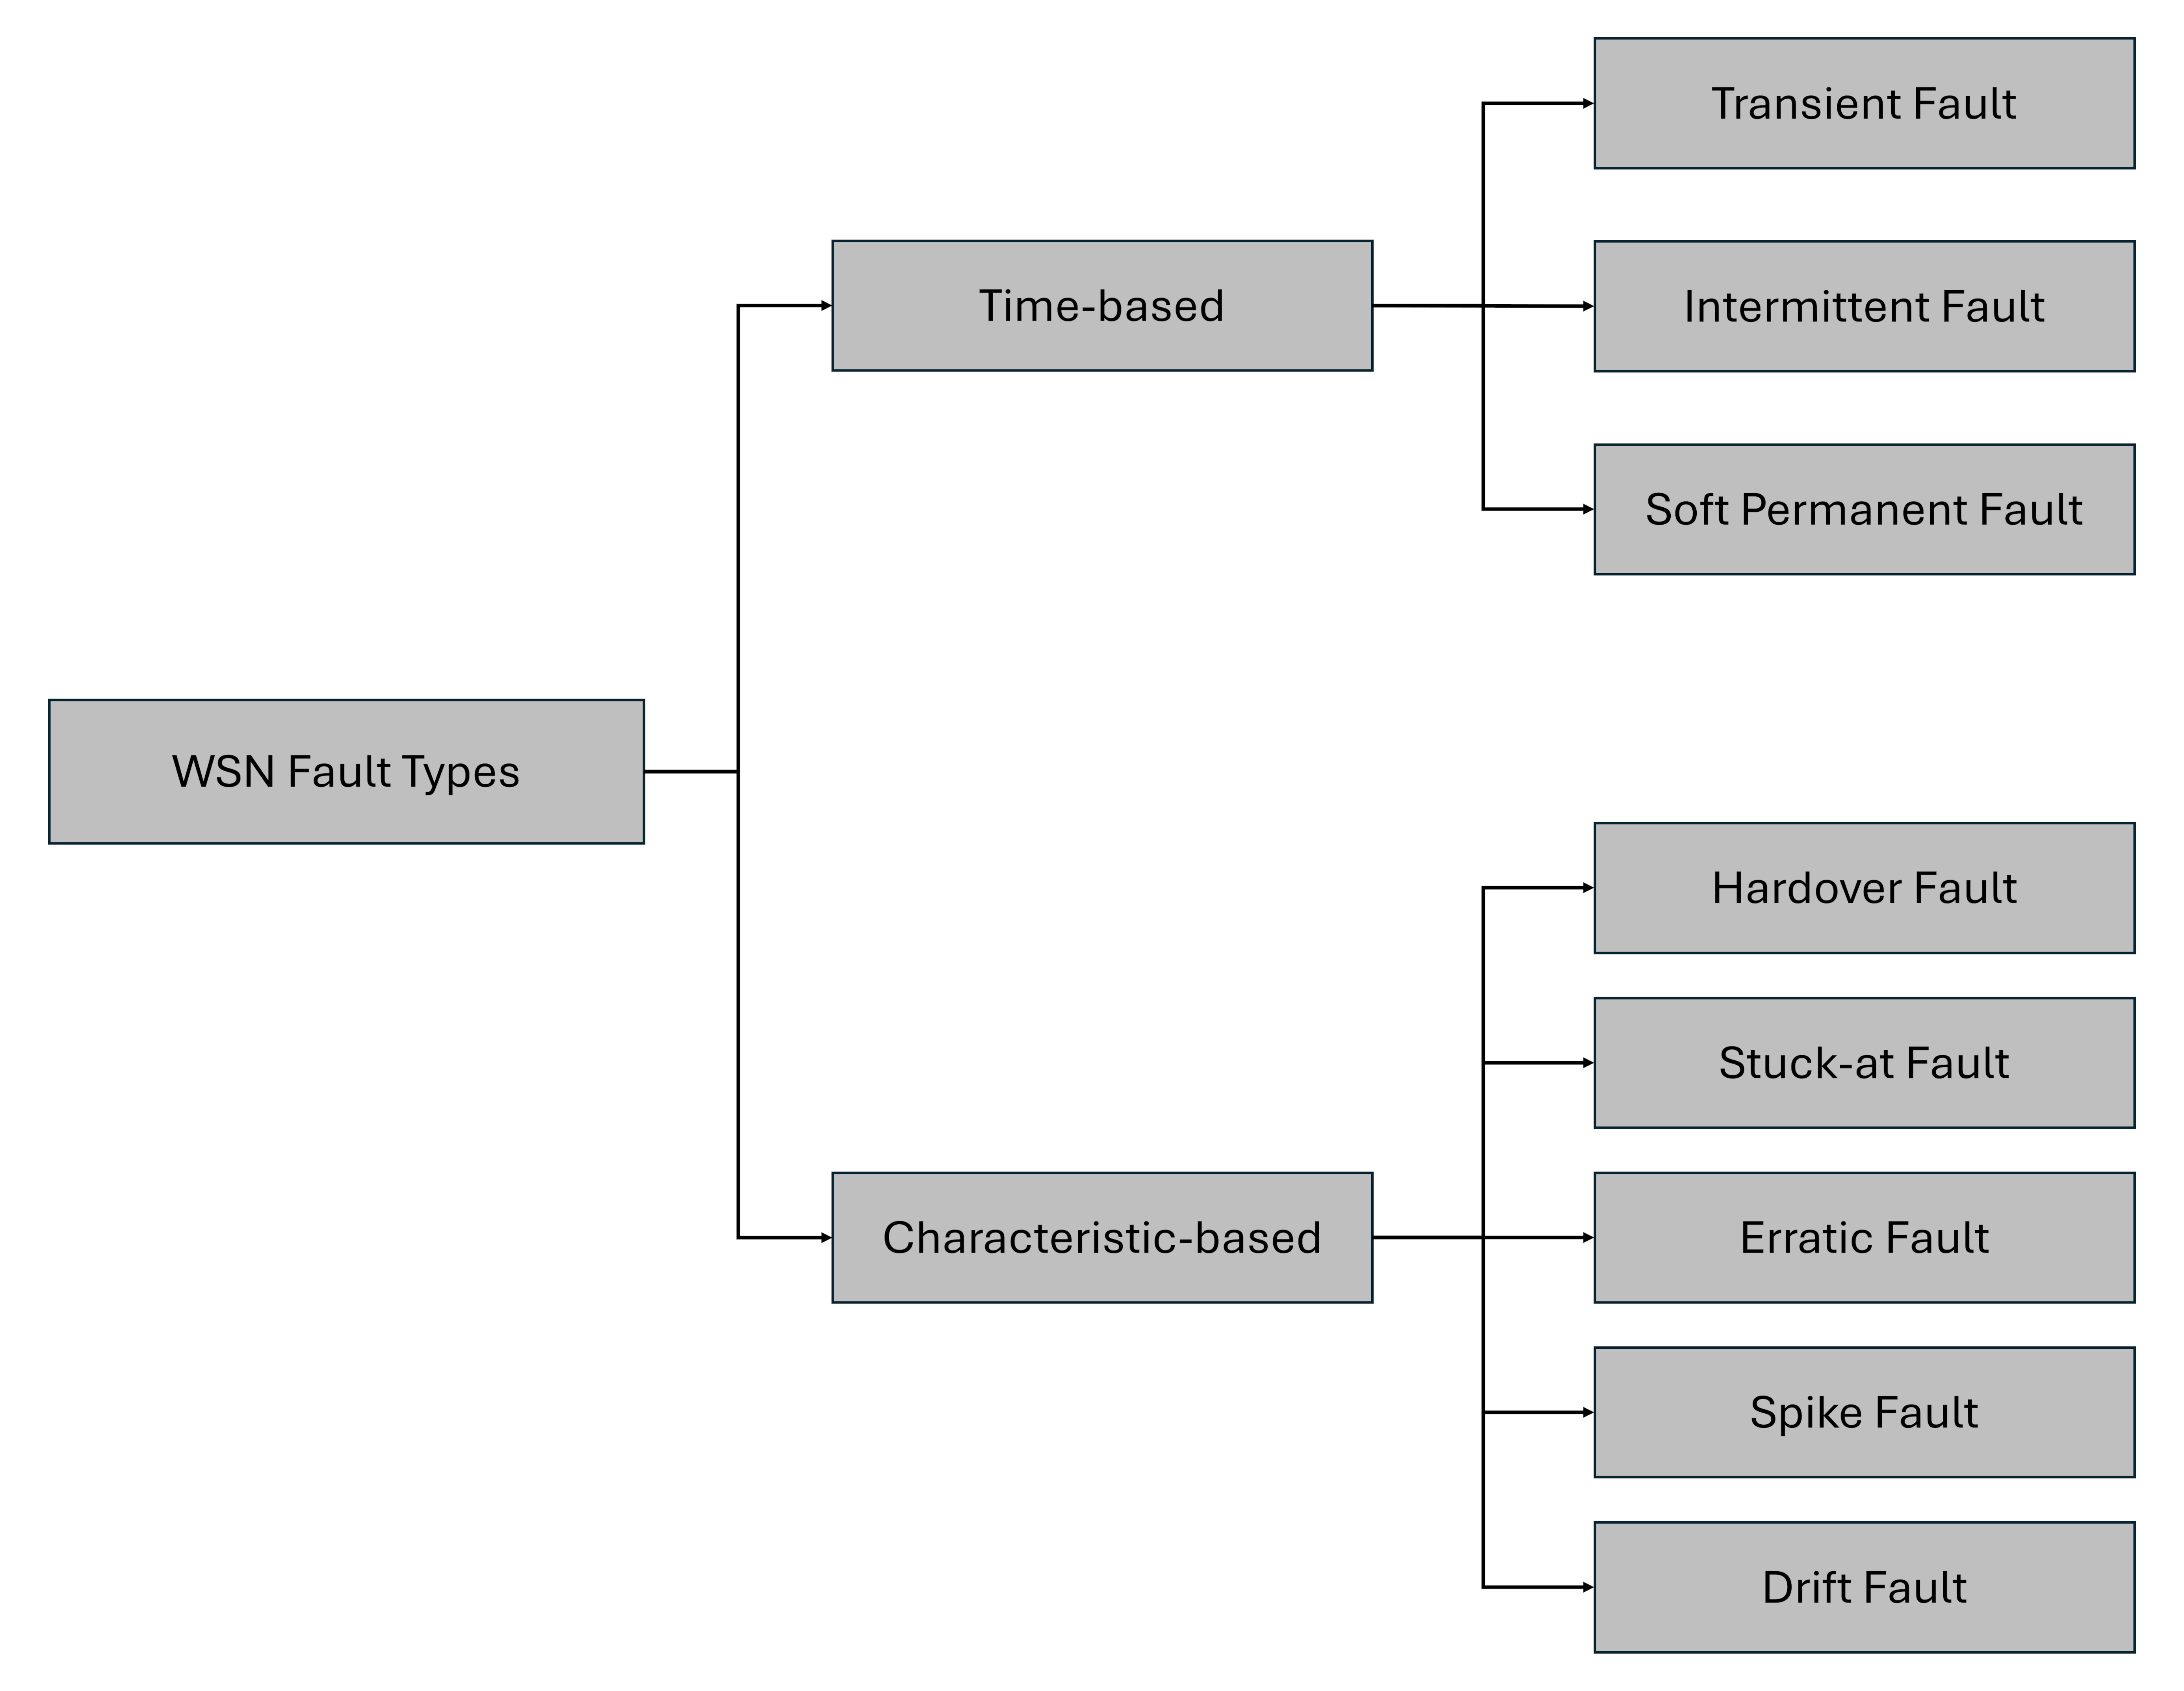
\includegraphics[width=\linewidth]{images/fault_taxonomy.png}
  \caption{WSN Fault Taxonomy}
  \label{fig:types}
\end{figure}

Existing fault detection methods in WSNs include model-based approaches, data-driven approaches and hybrid information-based methods \cite{Shi2024}. The most common approach is a model-based algorithm, which utilize mathematical and statistical principles to model each fault type. The data-driven approach on the other hand uses the analysis of data samples obtained to build a model for fault classification. Hybrid information-based methods use both human knowledge and data through a combination of different methods. Prior work either focuses on temporal patterns at individual nodes or spatial relations across neighbors, but fails to integrate both effectively. Given the complexity of WSN data and the potential for unknown fault patterns, data-driven approaches that can learn from data are particularly promising. Furthermore, a hierarchical architecture can effectively model both local temporal dynamics and broader spatial dependencies. In this work, we investigate the efficacy of a data-driven hierarchical method for WSNs fault diagnosis. The major contribution of this paper are as follows:

\begin{itemize}
  \item Introduce a novel Iterative Graph Network (IGN) that integrates Graph Attention Convolution with a custom Confidence Modulator(CM), dynamically refining node representations through iterative confidence propagation.
  \item Propose HiFiNet, a hierarchical network. HiFiNet first employs a Long Short-Term Memory based stacked autoencoder (LSTM-SAE) at the edge for temporal feature extraction and initial fault screening, followed by IGN for aggregating neighborhood information and refining fault diagnosis.
  \item Create a synthetic WSN dataset using NASA’s MERRA-2 reanalysis data as a substitute for real-world environmental sensor measurements and inject fault to it and Intel Lab Dataset \cite{Intel2004}.
  \item Evaluate performance including various metrics such as: accuracy, F1-score, precision on the aforementioned datasets, demonstrate improvement against methods in the literature.
\end{itemize}


\section{Literature Review}
Fault diagnosis in WSNs has been extensively studied using both traditional rule-based/statistical methods and machine learning (ML) techniques. In non-ML approaches, sensors often use fixed thresholds, mathematical models, or combinatorial tests to identify anomalies. For example, Panda et al. proposed a fault detection algorithm based on z-score function \cite{Panda2014}. Ahmad et al. proposed Kalman filtering as a lightweight anomaly detector in WSNs, but pure Kalman models degrade under fluctuating conditions \cite{Ahmad2024}. These methods typically require hand-tuned parameters and can yield high false alarms when environmental noise is high \cite{Muhammed2017, Zhang2018}. In contrast, ML-based approaches learn patterns from data. ML methods can automatically capture complex patterns in sensor readings, improving outlier detection without explicit rules. Saeed et al. implemented extremely randomized trees using data collected from Telos B motes and evaluate against support vector machine, multilayer perceptron, random forest, decision tree, and extra-trees \cite{Saeed2021}. ML models often achieve high detection accuracy and F1-scores, but require representative training data and incur higher computational cost.

WSN fault detection architectures are typically classified as centralized, distributed, or self-diagnosis schemes \cite{Takele2024, Prasad2023}. In centralized schemes, all sensor nodes send status reports or readings to a base station (sink), which performs fault analysis \cite{Panda2014}. This simplifies the detection logic but incurs high communication overhead: as the network scales, the sink must process many messages, leading to increased latency and limited real-time applicability \cite{Muhammed2017, Zhang2018}. By contrast, self-diagnosis has each node monitor its own status (e.g., battery level or sensor output) and detect local faults. Prasad et al. presented a deep belief network for time-based fault classification using each node data independently \cite{Prasad2023}. Distributed strategies involve neighbors or cluster-heads collaborating to detect faults. For example, nodes can mutually cross-check readings or vote on anomalies, and cluster-heads can aggregate data for local inference. These decentralized methods improve detection accuracy (errors are confirmed by multiple nodes) and scale better via clustering, but they consume extra energy and bandwidth for peer communication. In particular, Adday et al. note that cluster-based diagnosis can reduce communication relative to flat schemes and improve scalability \cite{Adday2022}.

Recent advances have explored hierarchical and hybrid techniques that fuse multiple levels of analysis and feature types. Hierarchical WSN architectures (e.g. clustering) naturally allow multi-stage diagnosis, where cluster-heads perform local detection and report to higher layers. Hybrid information-based method combine expert knowledge with quantitive data using many different algorithms. Shi et al. employed a belief rule base with adaptive attribute weights to improve on traditional static rule base \cite{Shi2024}. Importantly, this study emphasize that sensor data possess strong temporal and spatial correlations, and that fault features should capture both aspects. These efforts suggest a trend toward spatio-temporal fusion: e.g. using time-series prediction at each node together with spatial neighbor-consensus. Nevertheless, truly integrated models that jointly leverage per-node temporal dynamics and network-wide spatial context are still rare in the literature. HiFiNet is motivated by this gap, seeking to hierarchically combine temporal modeling (autoregressive encoding at nodes) with spatial modeling (graph-based fusion across nodes).


\section{System Model and Problem Statement}
\subsection{System Model}
We consider a WSN as an undirected graph \(G=(V,E))\), where \(V=\{v_1, v_2, \ldots, v_N\}\) is the set of \(N\) sensor nodes and \(E \subseteq V \times V\) represents bidirectional communication links between neighboring nodes. Each node \(v_i\) is equipped with a sensing modality and generates a time-series measurement \(x_i(t)\) at discrete time steps \(t=1, 2, \ldots, T\). Communication between \(v_i\) and \(v_j\) is possible if \((v_i,v_j) \in E\). 

This paper make the following additional assumptions:
\begin{itemize}
  \item Static or Slowly Varying Topology: Sensor nodes are assumed to be stationary or exhibit negligible mobility during the diagnosis window, so that network links \(E\) remain constant or change infrequently.
  \item Global Time Synchronization: Nodes maintain loosely synchronized clocks, ensuring measurements \(x_i(t)\) across the network align within a bounded jitter. 
  \item Existence of a Single High-Capacity Node/Sink: A base node with higher computation and memory resources is reachable (directly or multi-hop) from all nodes and knows the network topology apriori. 
\end{itemize}

\subsection{Fault Taxonomy}
\label{subsec:types}
Building upon the general categorization of faults, this section details the specific characteristic-based fault types that are the focus of our detection and diagnosis efforts. These faults represent common anomalies observed in WSN sensor readings and are well-documented in the literature \cite{Saeed2021, Hasan2024, Shi2024, Ni2009}. Understanding their distinct signatures is essential for designing robust fault detection and classification algorithms. The faults considered in this study are: hardover, drift, spike, erratic, and stuck-at fault. 

\subsubsection{Hardover Fault}
A hardover fault, also commonly referred to as a bias fault, occurs when the sensor's output signal experiences a sudden and persistent shift by a constant offset from its normal operational range \cite{Saeed2021, Shi2024, Hasan2024}. The sensor continues to respond to changes in the measured variable, but all readings are offset by this fixed amount. This can be caused by issues like calibration errors or a sudden change in the sensor's baseline. If \(S_\text{normal}(t)\) is the true sensor reading at time \(t\), the faulty signal, \(S_\text{hardover}(t)\), can be represented as:
\[S_\text{hardover}(t) = S_\text{normal}(t) + b\]
where \(b\) is a constant bias value \cite{Saeed2021}.

\subsubsection{Drift Fault}
A drift fault is characterized by a gradual and continuous deviation of the sensor readings from the true values over time \cite{Saeed2021, Hasan2024}. This deviation often manifests as a linear increase or decrease, though non-linear drifts are also possible. Drift can be caused by aging components, environmental changes affecting the sensor, or gradual degradation of sensor calibration. For a linear drift, the faulty signal, \(S_\text{drift}(t_n)\) at discrete time sample \(n\), can be modeled as:
\[S_\text{drift}(t_n) = S_\text{normal}(t_n) + n \cdot b_0\]
where \(n\) is the time index or sample number, and \(b_0\) is an initial constant drift rate \cite{Saeed2021}. Hasan et al. also model this as \(S_\text{drift}^N = S_\text{normal}^N +\beta^N\), where \(\beta^N\) represents the accumulated drift \cite{Hasan2024}.

\subsubsection{Spike Fault}
Spike faults are transient anomalies characterized by sudden, short-duration, large-magnitude deviations in sensor readings, after which the readings typically return to normal or near-normal values \cite{Saeed2021, Shi2024}. They appear as sharp peaks or impulses in the data stream. Spikes can be caused by electromagnetic interference, power supply glitches, or other transient disturbances. If \(S_\text{normal}(t)\) is the normal signal, a spike at time \(t_s\) might be represented as:
\[S_\text{spike}(t_s) = S_\text{normal}(t_s) + b_\text{spike}\]
where \(b_\text{spike}\) is a constant large value, and for \(t \neq t_s\), \(S_\text{spike}(t) \approx S_\text{normal}(t)\) \cite{Saeed2021, Shi2024}.

\subsubsection{Erratic Fault}
An erratic fault, sometimes referred to as precision degradation or increased noise, is characterized by sensor readings that exhibit random fluctuations of significantly increased amplitude around the true value \cite{Saeed2021}. While the average reading over a long period might still be close to the true value, the individual readings become highly unreliable due to the increased variance. This can be caused by failing sensor components, loose connections, or severe environmental interference. The faulty signal can be represented as:
\[S_\text{erratic}(t) = S_\text{normal}(t) + \eta(t)\]
where \(\eta(t)\) is a noise term with zero mean but significantly higher variance (\(\sigma_\text{erratic} \gg \sigma_\text{normal}\)) than the inherent sensor noise under normal operating conditions \cite{Saeed2021}.

\subsubsection{Stuck-at Fault}
A stuck-at fault (or stuck fault) occurs when the sensor output remains fixed at a constant value for a prolonged period, irrespective of any changes in the measured physical phenomenon \cite{Saeed2021, Hasan2024, Shi2024}. This constant value could be zero, a previous valid reading, the maximum or minimum of the sensor's range, or an arbitrary value. Common causes include complete sensor failure, signal clipping, or a disconnection in the data path. Mathematically, this is expressed as:
\[S_\text{stuck} = c\]
where \(c\) is a constant value, either from the nearest normal value or a random value \cite{Saeed2021, Hasan2024, Shi2024}.

% TODO: add sample figure for each fault types

\subsection{Problem Statement}
Given a segment of a sensor time series and a predefined set of fault classes, the problem is to assign the most appropriate fault class label to that time series segment.

Consider an input time series \(X_w = (x_t, x_{t+1}, \ldots, x_{t+w-1})\) of length \(w\), where \(x_i \in \mathbb{R}\) is the sensor reading at discrete time step \(i\). Define \(C = {c_1, c_2, \ldots, c_K}\) as the set of \(K\) mutually exclusive fault classes as detailed in the fault taxonomy (see \ref{subsec:types}) and the normal (fault-free) class.

The object is to learn a classification function (or hypothesis) \(h\) that maps the input feature vector \(\mathbf{x}\) (derived from \(X_w\)) to a predicted fault class label \(\hat{y}\ \in C\).


\section{Proposed Algorithm}
This section details the experimental methodology, including the dataset employed, the procedures for data pre-processing and synthetic fault injection, and the architecture of our proposed Hierarchical Fault Identification Network (HiFiNet) for fault classification in WSNs.

\subsection{Fault Injection}
To evaluate the performance of HiFiNet in classifying various fault types, synthetic faults were injected into the pre-processed normal temperature data. 

For each experimental dataset used, faults were injected such that within the selected subset of six nodes, five nodes were each assigned a distinct fault type, and one node remained normal. This setup allows for the analysis of one specific fault type per sensor in the context of other faulty and normal sensors.

Multiple datasets were generated with varying overall percentages of faulty instances, specifically 5\%, 10\%, 15\%, and 20\% of the total data points being faulty. Within each dataset, the total fault rate was divided equally among the five predefined fault types. Faults were injected based on their mathematical models Equation \ref{eq:hardover}, \ref{eq:drift}, \ref{eq:spike}, \ref{eq:erratic}, and \ref{eq:stuck}. In total, 4 datasets are created from each original dataset corresponding to each fault rate.

The time series sequences were labeled with a specific fault type if any sample within that sequence contained the corresponding injected fault. This creates a labeled dataset suitable for supervised learning.

\subsection{Hierarchical Fault Identification Network (HiFiNet)}
\begin{figure}
  \centering
  \includegraphics[width=0.65\linewidth]{images/HiFiNet.png}
  \caption{Proposed HiFiNet model, illustrating the Edge Classifier processing a target node's temperature sequence and the Network Classifier integrating edge outputs with contextual network data.}
  \label{fig:hifinet}
\end{figure}
We propose HiFiNet, a Hierarchical Fault Identification Network, for the classification of sensor faults in WSNs. The architecture, depicted in Figure~\ref{fig:hifinet}, employs a two-stage hierarchical approach to classify faults, leveraging both individual sensor data and contextual information from the network.

\subsubsection{Edge Classifier}
The first stage of HiFiNet is the Edge Classifier, which focuses on analyzing the time series data from an individual target sensor node to extract discriminative features and perform an initial fault classification. The design of the Edge Classifier involves a two-phase training process: unsupervised pre-training of a feature extractor using a LSTM-SAE architecture, followed by supervised fine-tuning for the fault classification task.

The feature-extraction component is built from an LSTM-SAE with encoder layers. In the first phase, this autoencoder is trained in an unsupervised, layer-wise fashion to learn compressed representations of \(X_w\). Define \(E_l(\cdot; \theta_{E_l})\) as the \(l\)-th LSTM encoder layer with parameters \(\theta_{E_l}\), \(D_l(\cdot; \theta_{D_l})\) as the corresponding decoder layer with parameters \(\theta_{D_l}\), and \(H_l\) as the hidden representation output by \(E_l\). We have:
\begin{itemize}
  \item \emph{Layer \(l=1\):}
    \begin{equation}
      \begin{aligned}
        H_1 &= E_1(X_w; \theta_{E_1}), \\
        \hat X_w &= D_1(H_1; \theta_{D_1}), \\
      \end{aligned}
    \end{equation}
    with \(\hat X_w\) being the reconstructed input. Then the objective is to optimize the reconstruction loss with respective to the network parameters:
    \begin{equation}
      (\hat \theta_{E_1},\,\hat \theta_{D_1}) = \underset{\theta_{E_1}, \theta_{D_1}} {\arg\min} \mathcal L_{\text{recon}}(X_w; \hat X_w)
    \end{equation}
  \item \emph{Layer \(l = 2, \ldots, L\)}

    Define \(H^*_{l-1}\) as the output of the \((l-1)\)-th trained encoder layer. We have:
    \begin{equation}
      \begin{aligned}
        H_l &= E_l(H^*_{L-1}; \theta_{E_l}), \\ 
        \hat H^*_{l-1} &= D_l(H_l; \theta_{D_l}), \\
      \end{aligned}
    \end{equation}
    with \(\hat H^*_{l-1}\) being the reconstructed input. Again the objective is to optimize the reconstruction loss with to the network parameters:
\begin{equation}
(\hat \theta_{E_l},\,\hat \theta_{D_l}) = \underset{\theta_{E_l}, \theta_{D_l}} {\arg\min} \mathcal L_{\text{recon}}(H^*_{l-1}; \hat H^*_{l-1})
\end{equation}
\end{itemize}
  After all \(L\) layers are pre-trained, the full stacked LSTM encoder is formed by concatenating these trained layers: \(E_\text{stacked}(\cdot; \Theta^*_{E}) = E_L(\ldots E_1(\cdot; \theta^*_{E_L}) \ldots;\theta^*_{E_L})\)
  
The pre-trained stacked LSTM encoder, \(E_\text{stacked}\), now served as the feature extractor for the Edge Classifier. In the second phase, classification head is attached to this encoder to create the Edge Classifier. The complete network is then trained using the labeled dataset.

\subsubsection{Iterative Graph Network}
The second stage of HiFiNet is the Network Classifier, which refines the initial fault assessments or embeddings from the Edge Classifier by incorporating network-wide spatial context and inter-node dependencies. The core of the Network Classifier is an IGN.

The IGN is designed to dynamically refine node representations by iteratively propagating and aggregating information across the graph, modulated by an evolving confidence measure. Let \(\mathcal{H}^{(0)} \in \mathbb{R}^{N \times d_0}\) be the vector representation of a node with \(N\) is the number of nodes and \(d_0\) is the dimension of the edge output. The IGN performs \(K\) iterations.

In each iteration \(k = 0, \dots, K\):
\begin{itemize}
    \item Feature Modulation (for \(k > 0\)):
      The initial node embeddings $\mathbf{H}^{(0)}$ are modulated based on a confidence score vector \(\mathbb{c}^{(k-1)} \in \mathbb{R}^{N \times 1}\), derived from the \((k-1)\)-th iteration's GAT output. A Confidence Modulator function, $\mathcal{M}_{\text{c}}$, is employed using Feature-wise Linear Modulation (FiLM):
\begin{equation}
\mathcal{H}'^{(k)} = \mathcal{M}_{\text{c}}(\mathcal{H}^{(0)}, \mathbb{c}^{(k-1)}) = g_{\gamma}(c^{(k-1)}) \odot \mathcal{H}^{(0)} + g_{\beta}(c^{(k-1)})
\end{equation}
    where \(g_{\gamma}(\cdot)\) and \(g_{\beta}(\cdot)\) are learnable functions that generate scaling and shifting parameters from the confidence scores, and \(\odot\) denotes element-wise multiplication. For the first iteration \(k=0\), no modulation is applied, so \(\mathcal{H}'^{(0)} = \mathcal{H}^{(0)}\). The Confidence Modulator allows the network to adaptively emphasize or de-emphasize features based on the current confidence in their classification.

    \item Graph Attention Convolution (GAT) Block:
    The modulated features \(\mathbb{H}'^{(k)}\) are then processed by a GAT block, denoted as \(\mathcal{G}\). This block typically consists of one or more Graph Attention Convolution layers, which enable nodes to selectively attend to their neighbors' features when updating their own representations:
\begin{equation}
\mathcal{H}_{\text{G}}^{(k)} = \mathcal{G}(\mathcal{H}'^{(k)}, A)
\end{equation}
    where \(A\) is the adjacency matrix representing the graph structure. Each GAT layer computes attention coefficients for neighboring nodes, aggregates their features weighted by these coefficients, and applies a linear transformation. Layer normalization and activation functions  are often applied between GAT layers. Dropout are also used for regularization. The output \(\mathcal{H}_{\text{G}}^{(k)} \in \mathbb{R}^{N \times d_{\text{G}}}\) contains node representations that have incorporated information from their local graph neighborhood.

    \item Temporary Classification and Confidence Update (if \(k < K-1)\):
    If it is not the final iteration, the output \(\mathcal{H}_{\text{G}}^{(k)}\) is passed through a temporary classifier, \(f_{\text{temp}}\), to obtain intermediate class logits \(z^{(k)}\) for each node:
\begin{equation}
z^{(k)} = f_{\text{temp}}(\mathcal{H}_{\text{G}}^{(k)})
\end{equation}
    These logits are converted to probabilities $P^{(k)}$ using the softmax function:
\begin{equation}
P^{(k)} = \text{softmax}(\mathbf{z}^{(k)})
\end{equation}
    The confidence score $c_i^{(k)}$ for each node $i$ is then derived from these probabilities, typically as the maximum probability value:
\begin{equation} 
c_i^{(k)} = \max(P_i^{(k)})
\end{equation}
    This results in a confidence vector $\mathbf{c}^{(k)}$, which is then used in the Feature Modulation step of the next iteration ($k+1$). This iterative process allows the model to progressively refine its understanding by focusing subsequent GAT operations based on the certainty of intermediate predictions.
\end{itemize}

After \(K\) iterations, the final GAT output $\mathcal{H}_{\text{G}}^{(K_{iter}-1)}$ represents the spatially-refined node embeddings. This and the original representation are then passed to a classification head to output the network classification.


\section{Experiments and Result}
In this section, we evaluated our proposed method against other methods in the literature. From previous research about fault diagnosis in WSNs, we selected  Deep Belief Network \cite{Prasad2023}, LSTM-AE \cite{Khan2024}, and Support Vector Machine(SVM).

\subsection{Dataset}
For purpose of fault detection, we created an original dataset using data from NASA MERRA-2 reanalysis data (Temperature at 2 Meter) as substitution for measurements taken from a WSN \cite{GMAO2015}. The data is collected from the North Vietnam region from a period of roughly 6 months. Another dataset used for performance evaluation is the Intel Lab Dataset. This dataset comprises readings from a network of 54 sensor nodes, specifically Mica2Dot devices, which were outfitted with environmental sensing capabilities. These nodes systematically captured time-stamped information relating to ambient conditions, including temperature, humidity, light levels, and the sensors' own voltage. The data acquisition process occurred at intervals of roughly 31 seconds for each sensor. The collection period for this particular dataset extended from late February 2004 through early April 2004 \cite{Intel2004}.

\subsection{Metrics}
To evaluate the performance of the proposed HiFiNet and compare it with other methods, several standard classification metrics are employed. These metrics are calculated based on the number of true positives (TP), false positives (FP), true negatives (TN), and false negatives (FN) for each class. In a multi-class classification problem, these are often computed for each class $c_i$ in a set of classes $C = \{c_1, c_2, \dots, c_K\}$.

Given that \(TP_i\) is the number of true positives for class \(c_i\), \(FP_i\) is the number of false positives for class \(c_i\), \(FN_i\) is the number of false negatives for class \(c_i\), \(N\) is the total number of instances, \(N_i\) is the number of true instances belonging to class \(c_i\).

Accuracy measures the overall correctness of the classifier. It is the ratio of the number of correctly classified instances to the total number of instances.
\begin{equation}
  \text{Accuracy} = \frac{\sum_{i=1}^{K} TP_i}{N}
\end{equation}

Next, precision measures the proportion of positively predicted instances for class \(c_i\) that were actually correct. It is calculated as the ratio of true positives for class \(c_i\) to the sum of true positives and false positives for class \(c_i\).
\begin{equation}
  \text{Precision}_i = \frac{TP_i}{TP_i + FP_i}
\end{equation}
The weighted average precision is computed as:
\begin{equation}
  \text{Weighted Precision} = \sum_{i=1}^{K} \left( \frac{N_i}{N} \times \text{Precision}_i \right)
\end{equation}

Finally, the F1-score is the harmonic mean of precision and recall for a class \(c_i\), providing a single score that balances both concerns.
\begin{equation}
  \text{F1-score}_i = 2 \times \frac{\text{Precision}_i \times \text{Recall}_i}{\text{Precision}_i + \text{Recall}_i}
\end{equation}
Similarly, the weighted average F1-score is calculated by:
\begin{equation}
  \text{Weighted F1-score} = \sum_{i=1}^{K} \left( \frac{N_i}{N} \times \text{F1-score}_i \right)
\end{equation}

\subsection{Experiment Settings}
All experiment is implemented in Python and run inside Kaggle Notebook with a P100 GPU.

\subsection{Evaluation Result}
The overall classification accuracy, shown in Figure~\ref{fig:accuracy}, demonstrates a substantial uplift from HiFiNet. HiFiNet maintains a \(2\sim6\%\) accuracy advantage over the second-best model LSTM-AE. SVM and DBN lag behind with sub \(90\%\) and sub \(80\%\) accuracies respectively across datasets. More importantly, the accuracy of HiFiNet does not degrade significantly as fault rate increases when compared to other methods. This indicates that information from neighbors collected in HiFiNet has a major impact in stabilizing the performance when noise becomes more prevalent

\begin{figure}
  \centering
  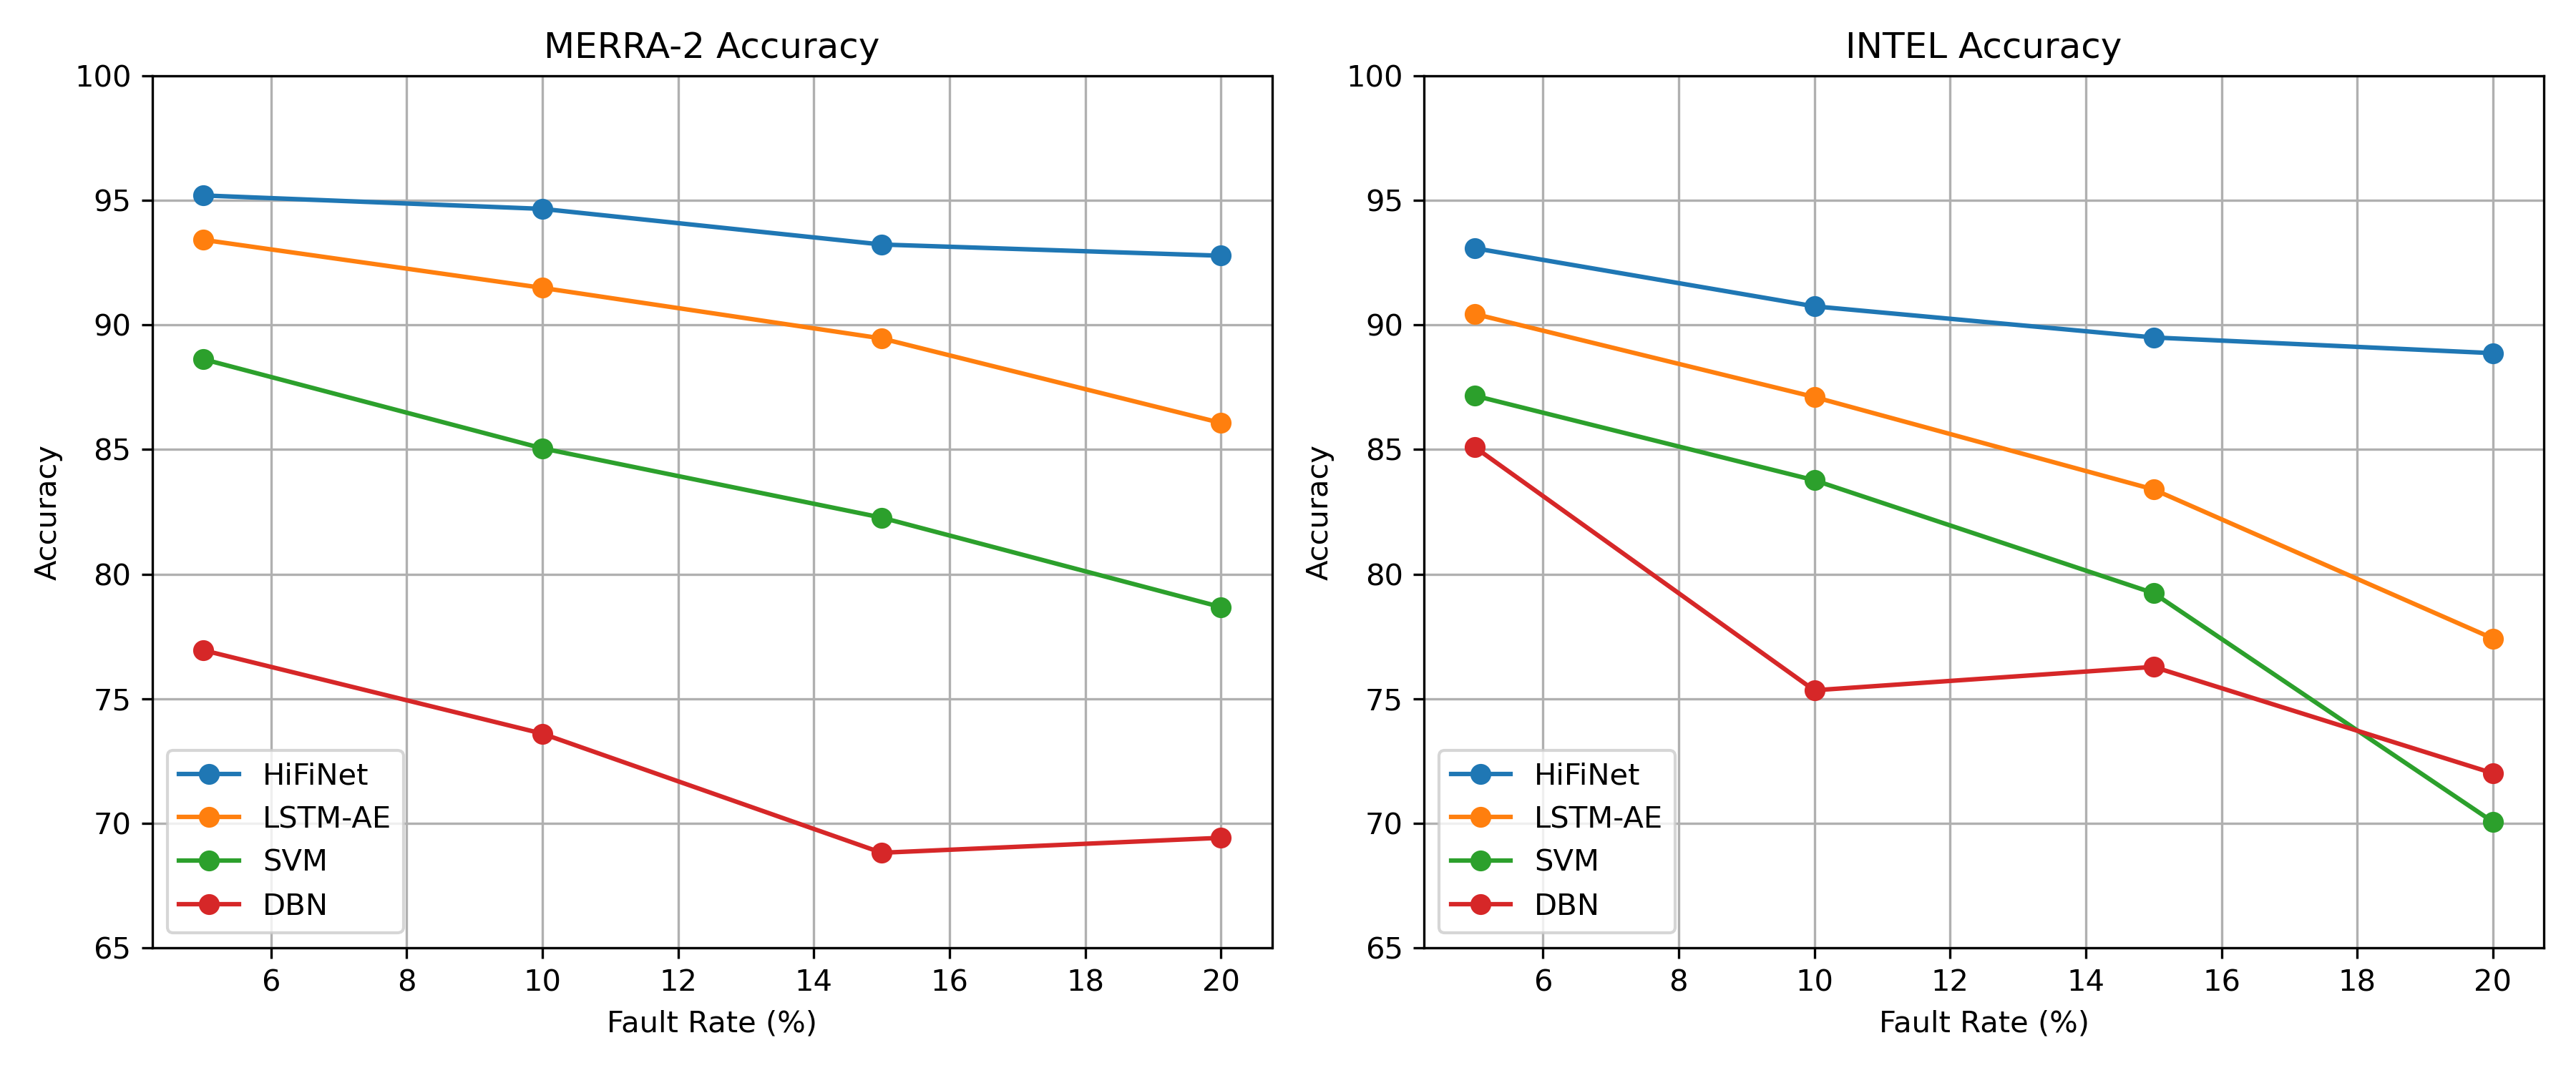
\includegraphics[width=\linewidth]{images/accuracy.png}
  \caption{Accuracy versus Fault Rate comparison between HiFiNet and other methods.}
  \label{fig:accuracy}
\end{figure}

Figure~\ref{fig:f1} plots the F1-Score against the rising fault rates. This further reinforce HiFiNet robustness under noisy condition. HiFiNet achieve upwards of \(94.70\%\) and \(92.32\%\) for MERRA-2 and Intel \(5\%\) fault rate datasets respectively. Compare to LSTM-AE, SVM and DBN, this means a performance delta of \(2\)-\(20\%\) and \(4\)-\(16\%\) on the corresponding datasets, with other fault rate datasets following a similar story. These results suggest that temporal and spatial features utilization has contributes significantly to HiFiNet ability to accurately diagnose each class.

\begin{figure}
  \centering
  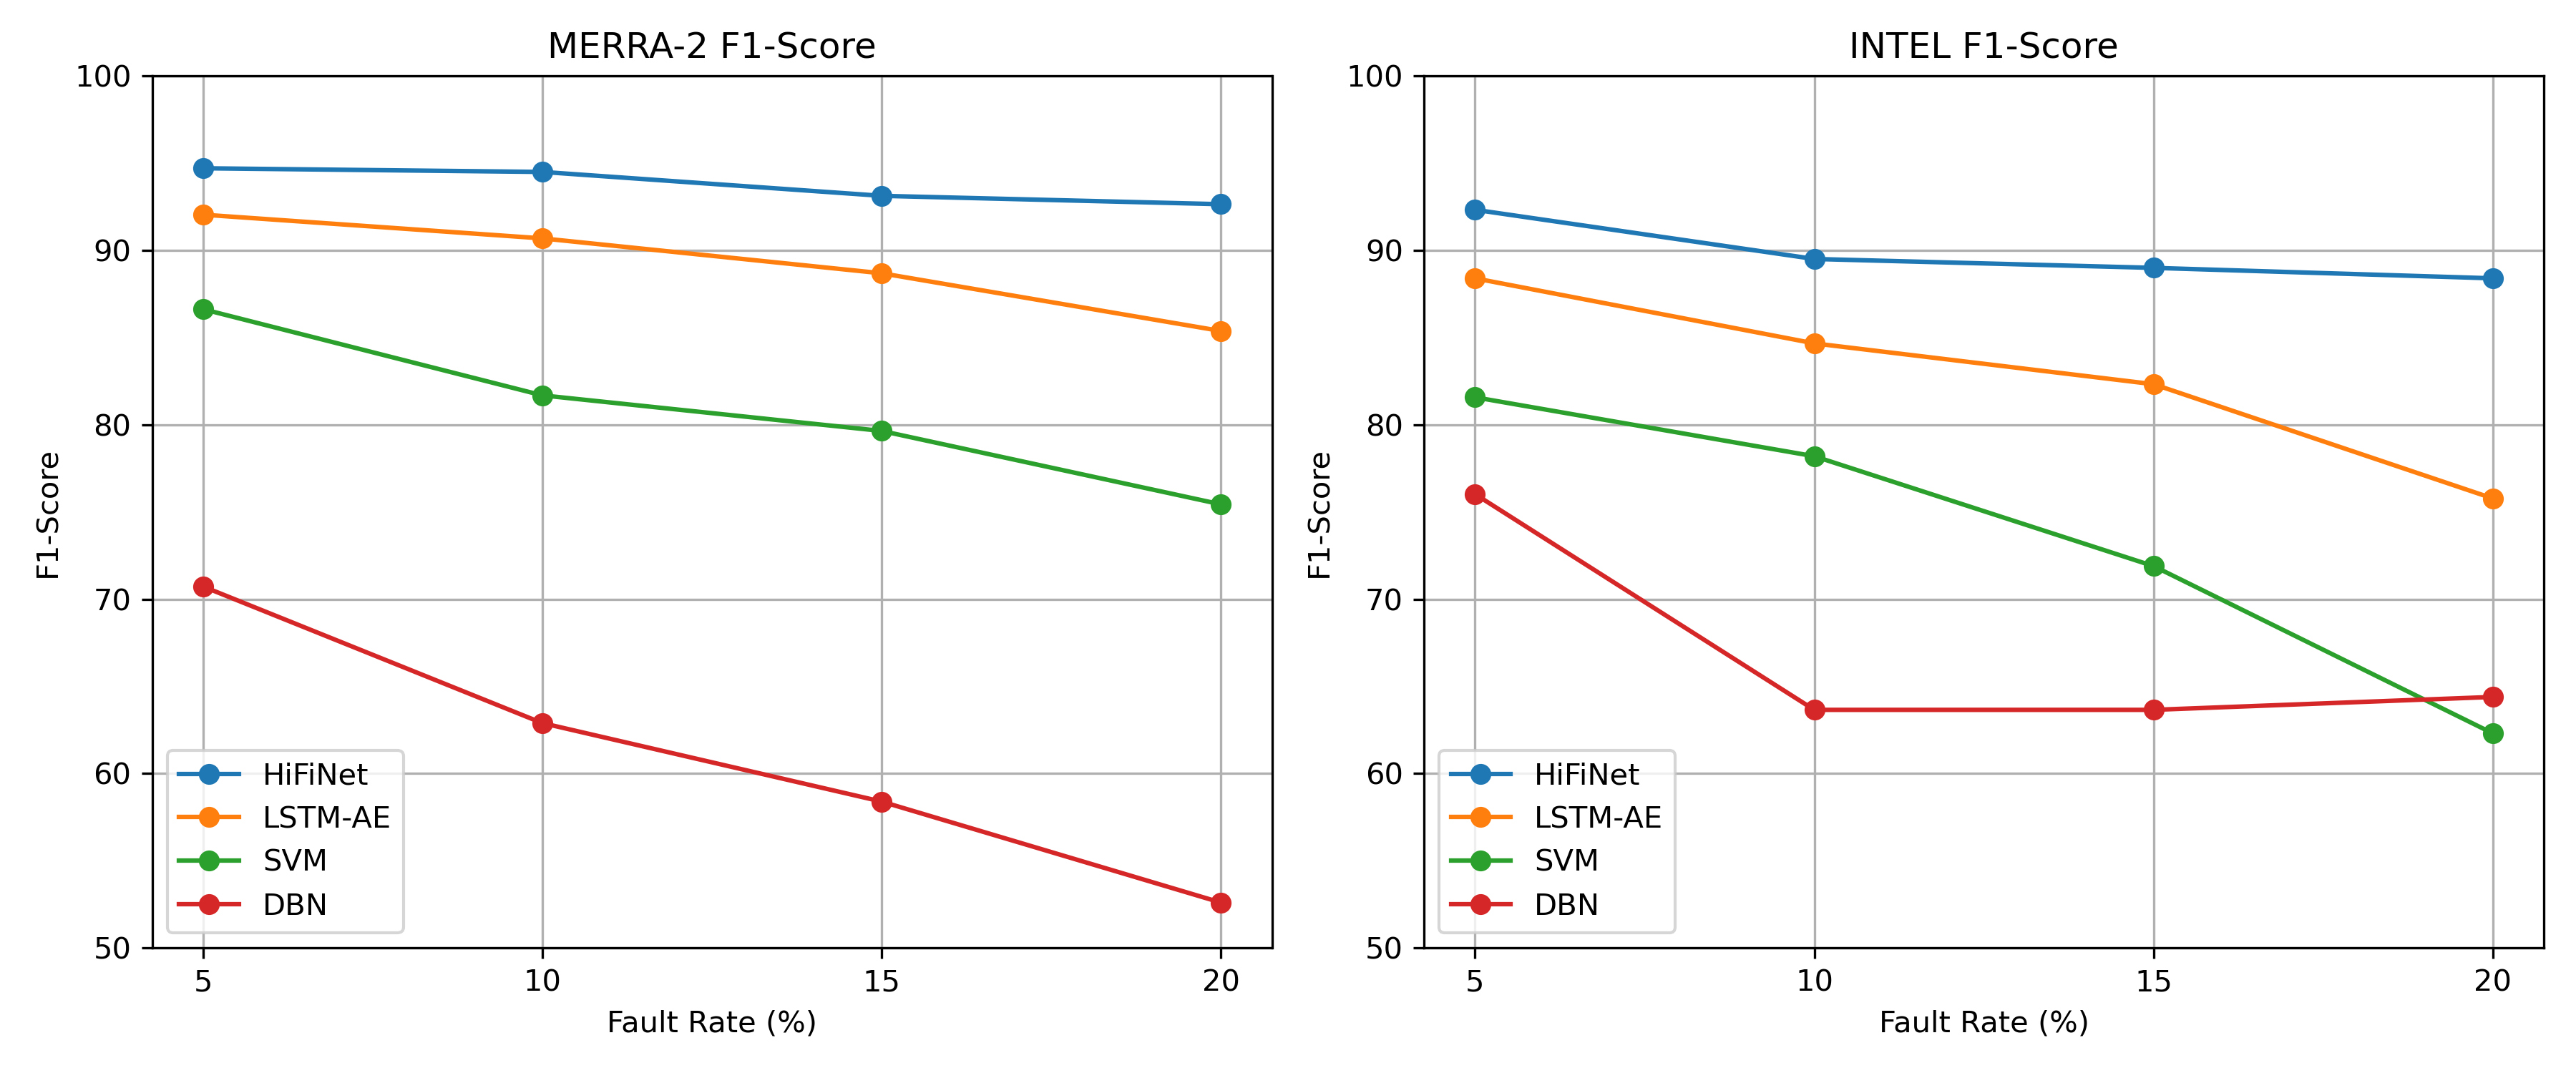
\includegraphics[width=\linewidth]{images/f1.png}
  \caption{F1-Score versus Fault Rate comparison between HiFiNet and other methods.}
  \label{fig:f1}
\end{figure}

To dissect the components of the F1-score, Figure~\ref{fig:pr_scatter} plots Precision versus Recall at the highest stress level (20\% fault rate). An ideal classifier would reside in the top-right corner, signifying perfect precision and recall. For both datasets, HiFiNet is positioned closest to this ideal point. This demonstrates that even in a highly corrupted environment, HiFiNet maintains a superior balance, successfully identifying a high proportion of actual faults (high recall) while simultaneously minimizing the number of false alarms (high precision).

\begin{figure}
  \centering
  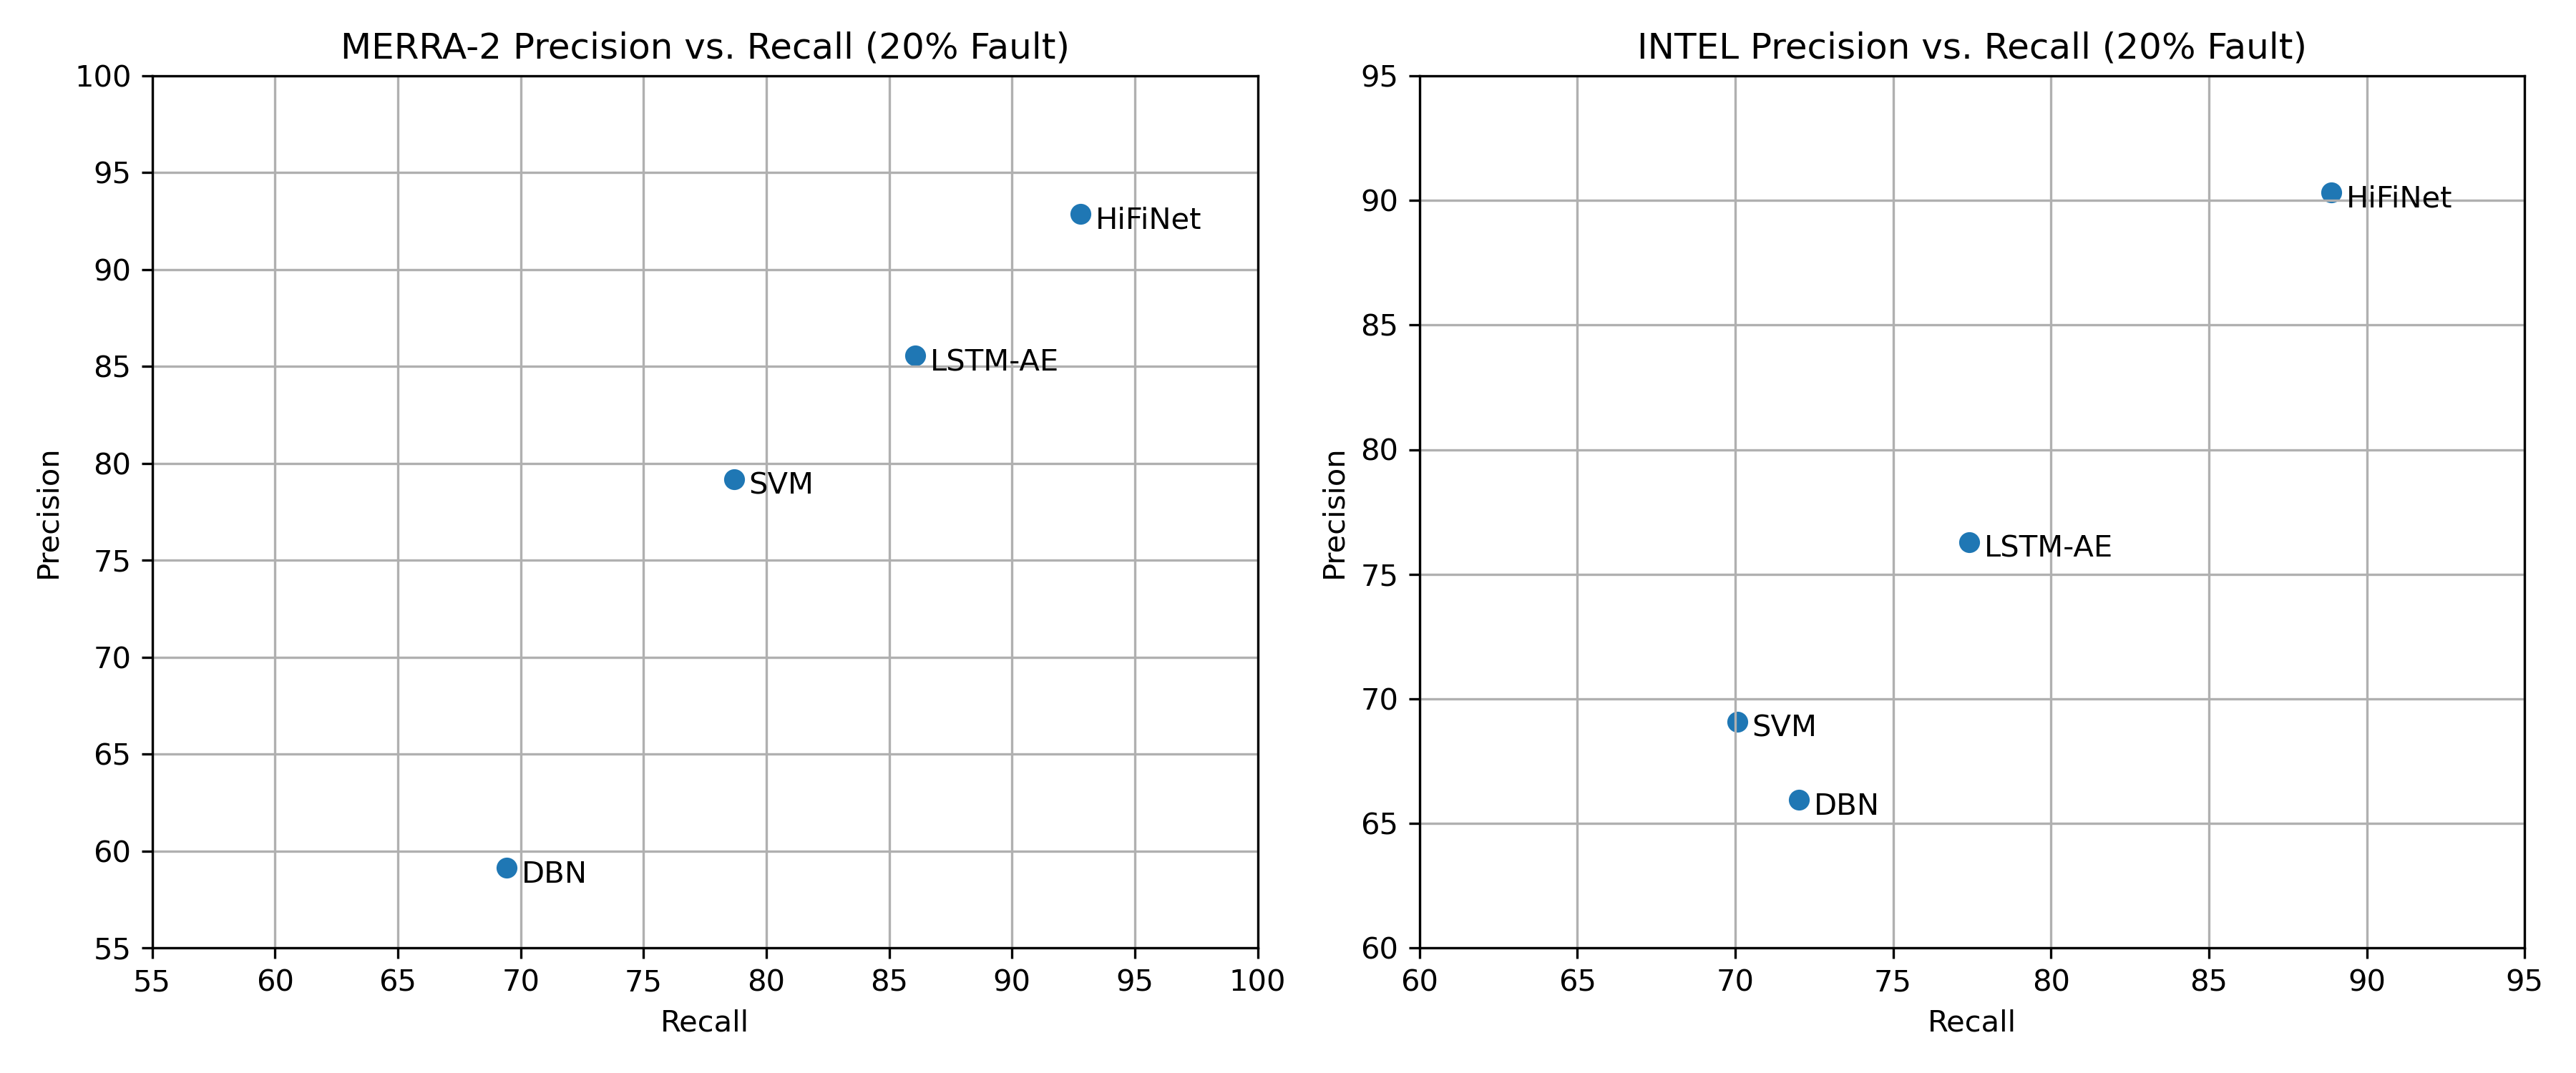
\includegraphics[width=\linewidth]{images/pr_scatter.png}
  \caption{Precision-Recall scatter plot comparison between HiFiNet and other methods. Weight-Average Recall is always equal to Total Accuracy}
  \label{fig:pr_scatter}
\end{figure}

Next, Figure~\ref{fig:f1_drop} provides a direct, quantitative measure of model stability. It visualizes the absolute drop in F1-Score as the fault rate increases from 5\% to 20\%. A smaller bar indicates greater robustness against worsening data quality. HiFiNet clearly stands out with the smallest performance drop on both datasets (2.06 points for MERRA-2 and 3.93 for INTEL). In contrast, models like SVM and LSTM-AE experience much larger drops, exceeding 11 and 12 points, respectively. This bar chart offers a stark visual confirmation of HiFiNet's superior stability and reliability under varying conditions.

\begin{figure}
  \centering
  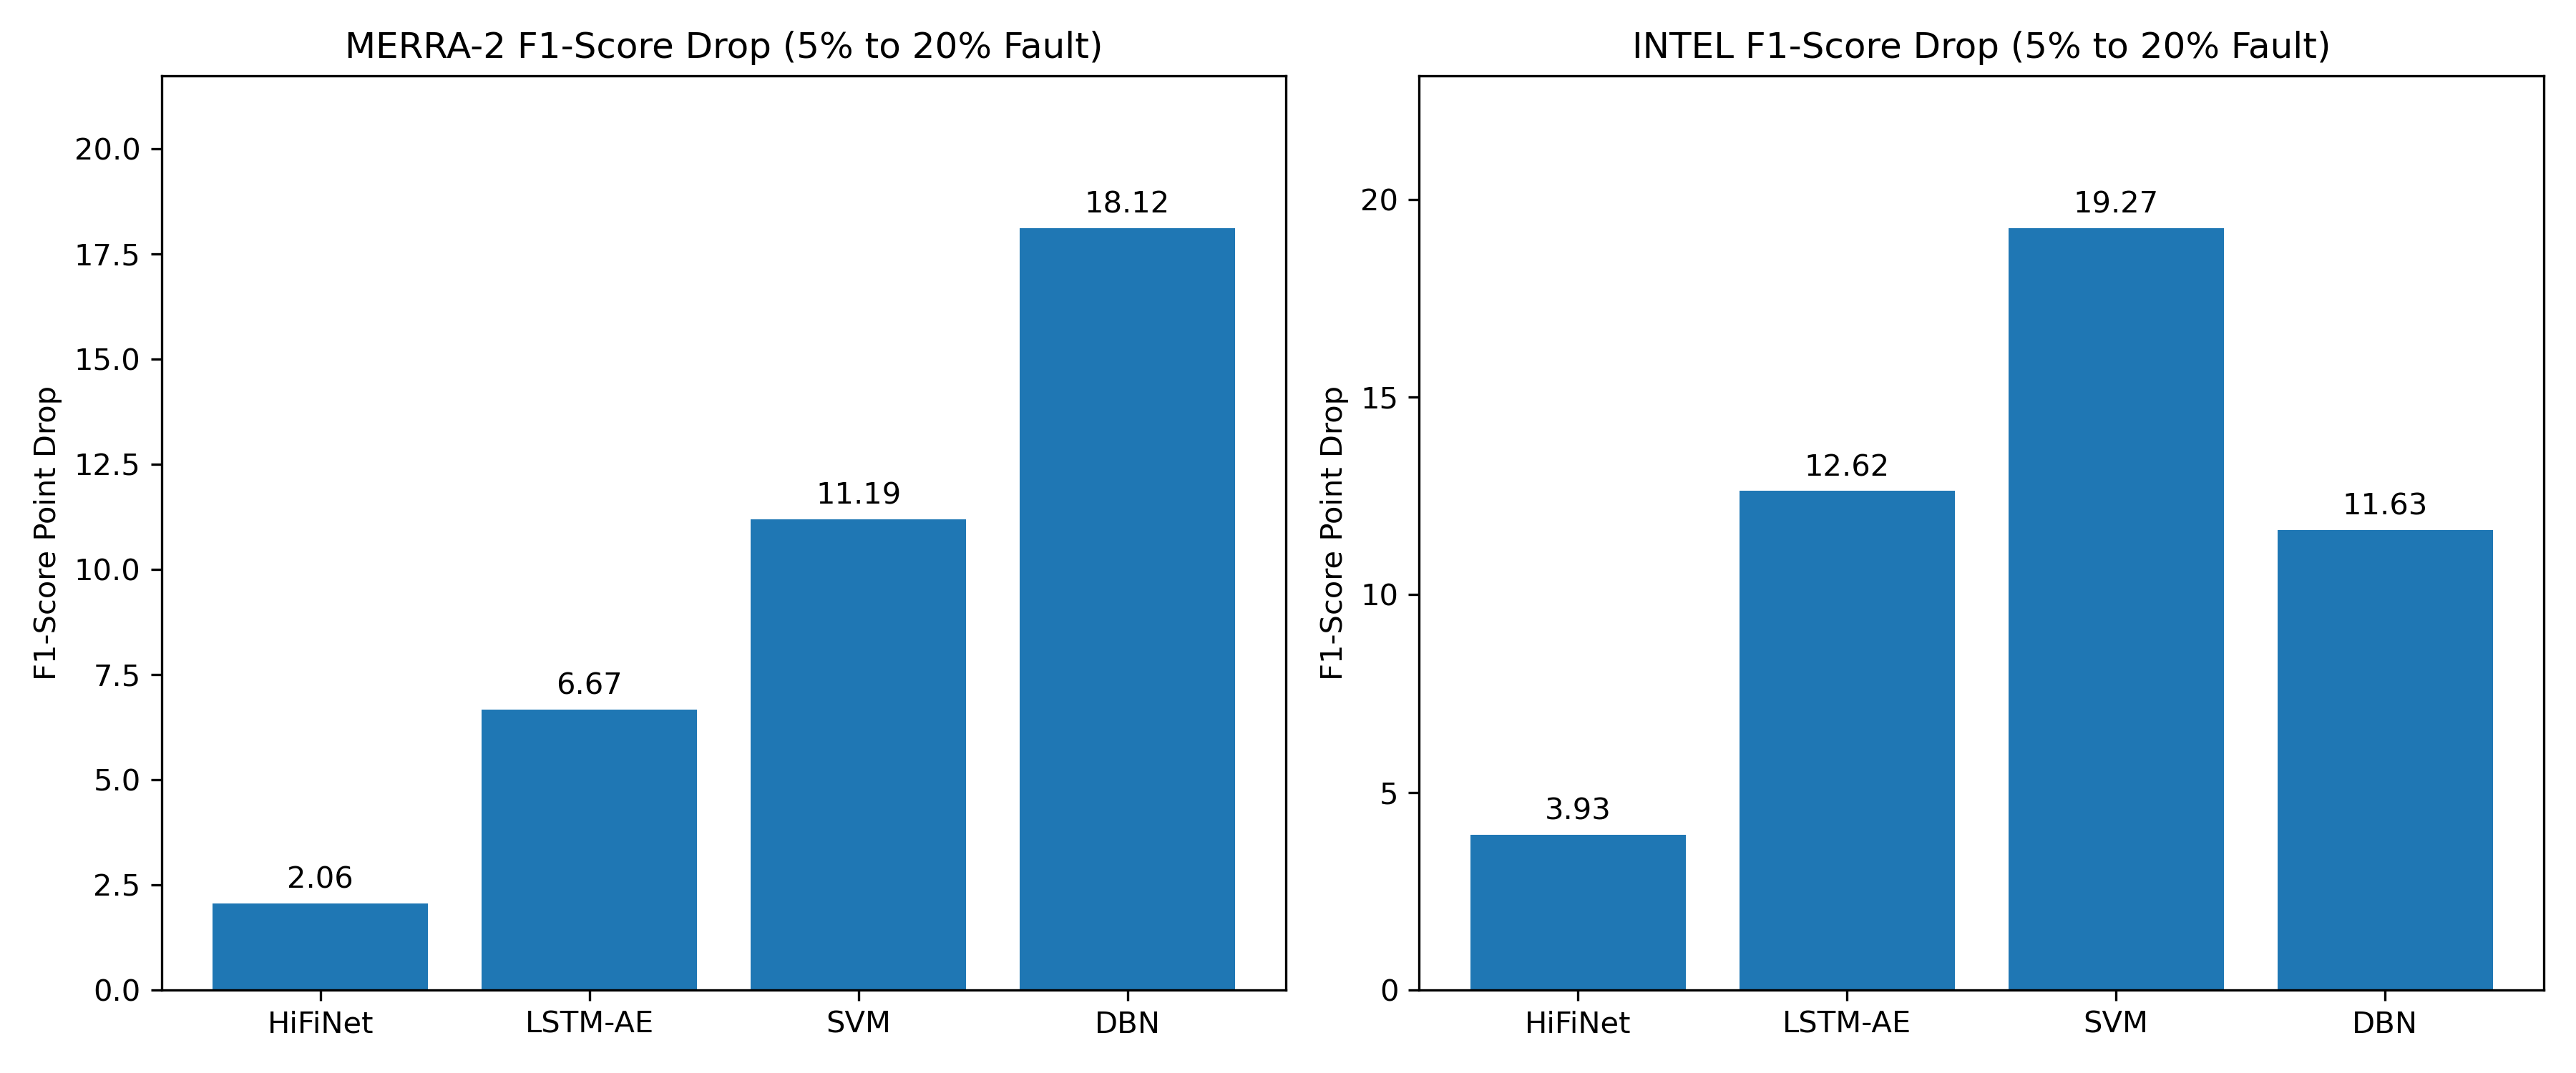
\includegraphics[width=\linewidth]{images/f1_drop.png}
  \caption{F1-Score drop comparison between HiFiNet and other methods.}
  \label{fig:f1_drop}
\end{figure}

While the previous figures provide a visual analysis of key performance trends, tHe complete numerical results for all metrics are consolidated in Table~\ref{tab:metrics} for reference.

\begin{table}
  \centering
  \resizebox{\linewidth}{!}{%
    \begin{tabular}{@{}llrrrrrrrr@{}}
      \toprule
      & & \multicolumn{4}{c}{MERRA-2} & \multicolumn{4}{c}{INTEL} \\
      \cmidrule(lr){3-6} \cmidrule(lr){7-10}
      Metric & Model & 5\% & 10\% & 15\% & 20\% & 5\% & 10\% & 15\% & 20\% \\
      \midrule
      \multirow{4}{*}{Accuracy}
      & HiFiNet   & \textbf{95.20} & \textbf{94.66} & \textbf{93.23} & \textbf{92.78} & \textbf{93.08} & \textbf{90.75} & \textbf{89.50} & \textbf{88.87} \\
      & LSTM-AE   & 93.42 & 91.49 & 89.46 & 86.07 & 90.44 & 87.11 & 83.40 & 77.42 \\
      & SVM       & 88.63 & 85.05 & 82.27 & 78.68 & 87.16 & 83.77 & 79.24 & 70.06 \\
      & DBN       & 76.95 & 73.60 & 68.82 & 69.42 & 85.09 & 75.34 & 76.28 & 72.01 \\
      \midrule
      \multirow{4}{*}{F1-Score}
      & HiFiNet   & \textbf{94.70} & \textbf{94.49} & \textbf{93.12} & \textbf{92.64} & \textbf{92.32} & \textbf{89.50} & \textbf{88.99} & \textbf{88.39} \\
      & LSTM-AE   & 92.04 & 90.68 & 88.68 & 85.37 & 88.39 & 84.66 & 82.32 & 75.77 \\
      & SVM       & 86.62 & 81.68 & 79.64 & 75.43 & 81.57 & 78.19 & 71.89 & 62.30 \\
      & DBN       & 70.72 & 62.89 & 58.39 & 52.60 & 76.02 & 63.65 & 63.65 & 64.39 \\
      \midrule
      \multirow{4}{*}{Precision}
      & HiFiNet   & \textbf{95.21} & \textbf{94.52} & \textbf{93.55} & \textbf{92.89} & \textbf{92.55} & \textbf{91.76} & \textbf{90.16} & \textbf{90.32} \\
      & LSTM-AE   & 92.10 & 90.90 & 89.35 & 85.55 & 89.53 & 86.63 & 82.71 & 76.28 \\
      & SVM       & 86.95 & 82.78 & 81.62 & 79.20 & 76.89 & 73.96 & 67.30 & 69.08 \\
      & DBN       & 70.47 & 60.98 & 53.12 & 59.14 & 72.43 & 66.77 & 57.48 & 65.95 \\
      \bottomrule
    \end{tabular}
  }
  \caption{Comprehensive performance metrics of each method on all datasets.}
  \label{tab:metrics}
\end{table}

\subsection{Ablation Study: Accuracy Tradeoff versus Energy Efficiency of HiFiNet}
This analysis investigates the crucial trade-off between the accuracy gained by incorporating neighborhood data and the energy consumed in the process, a primary concern in resource-constrained WSNs. The study's goal is to provide insight into how HiFiNet can be configured for different operational requirements, balancing diagnostic performance with network lifetime.

To quantify the energy cost, we adopt a widely used energy model for WSNs. The model accounts for the energy dissipated during signal transmission, reception, and processing. The combined energy for receiving, aggregating and transmitting data from node \(i\) to node \(j\) is defined by:
\begin{equation}
  E_{t_{ij}} = l (\epsilon_{elec} + \epsilon_{da} + \epsilon_{fs} \cdot d^2_{ij}),
\end{equation}
where \(d_{ij}\) is the distance between nodes \(i\) and \(j\), \(l\) is the number of bits, and \(\epsilon_{elec}\), \(\epsilon_{fs}\), and \(\epsilon_{da}\) represent the energy per bit dissipated in the electronic circuitry of the transmitter or the receiver, the energy cost of transmitting one bit of data over a unit distance squared at short distance, and the energy to aggregate one bit of data.

In our model, we use standard parameter values where \(\epsilon_{elec} = 50\) \si{nJ/bit}, \(\epsilon_{fs} = 10\) \si{pJ/bit/m^2}, \(\epsilon_{mp} = 0.0013\) \si{pJ/bit/m^4}, and the data aggregation energy cost \(\epsilon_{da} = 5 \) \si{nJ/bit}. We define Energy Efficiency (EE) as the inverse of the total energy spent:
\begin{equation}
  EE = 1 / E_{total}.
\end{equation}

The ablation study compares the full HiFiNet architecture against its baseline component: the Edge Classifier operating in isolation (i.e., without the Network Classifier's spatial aggregation). The Accuracy Delta (\%) measures the performance improvement provided by the full HiFiNet over this baseline. We introduce a tunable parameter, Time Delay \(t\), which represents the frequency of execution for the Network Classifier. A time delay of \(t=0\) means the spatial aggregation is performed for every time window processed by the Edge Classifier. A delay of \(t=k\) means the aggregation is performed only once every \(k+1\) time windows. The network is assumed to adopt the Constrained Application Protocol (CoAP) with a transmission overhead of 32 bytes.

The results of this trade-off are presented in Figure~\ref{fig:accuracy_tradeoff}. At a time delay of \(t=0\), the system performs continuous spatial aggregation. This yields the maximum diagnostic benefit, with HiFiNet achieving an Accuracy Delta of over \(3.1\%\) compared to the edge-only model. This configuration, however, is the most energy-intensive, resulting in the lowest Energy Efficiency (approx. 40 units).

\begin{figure}
  \centering
  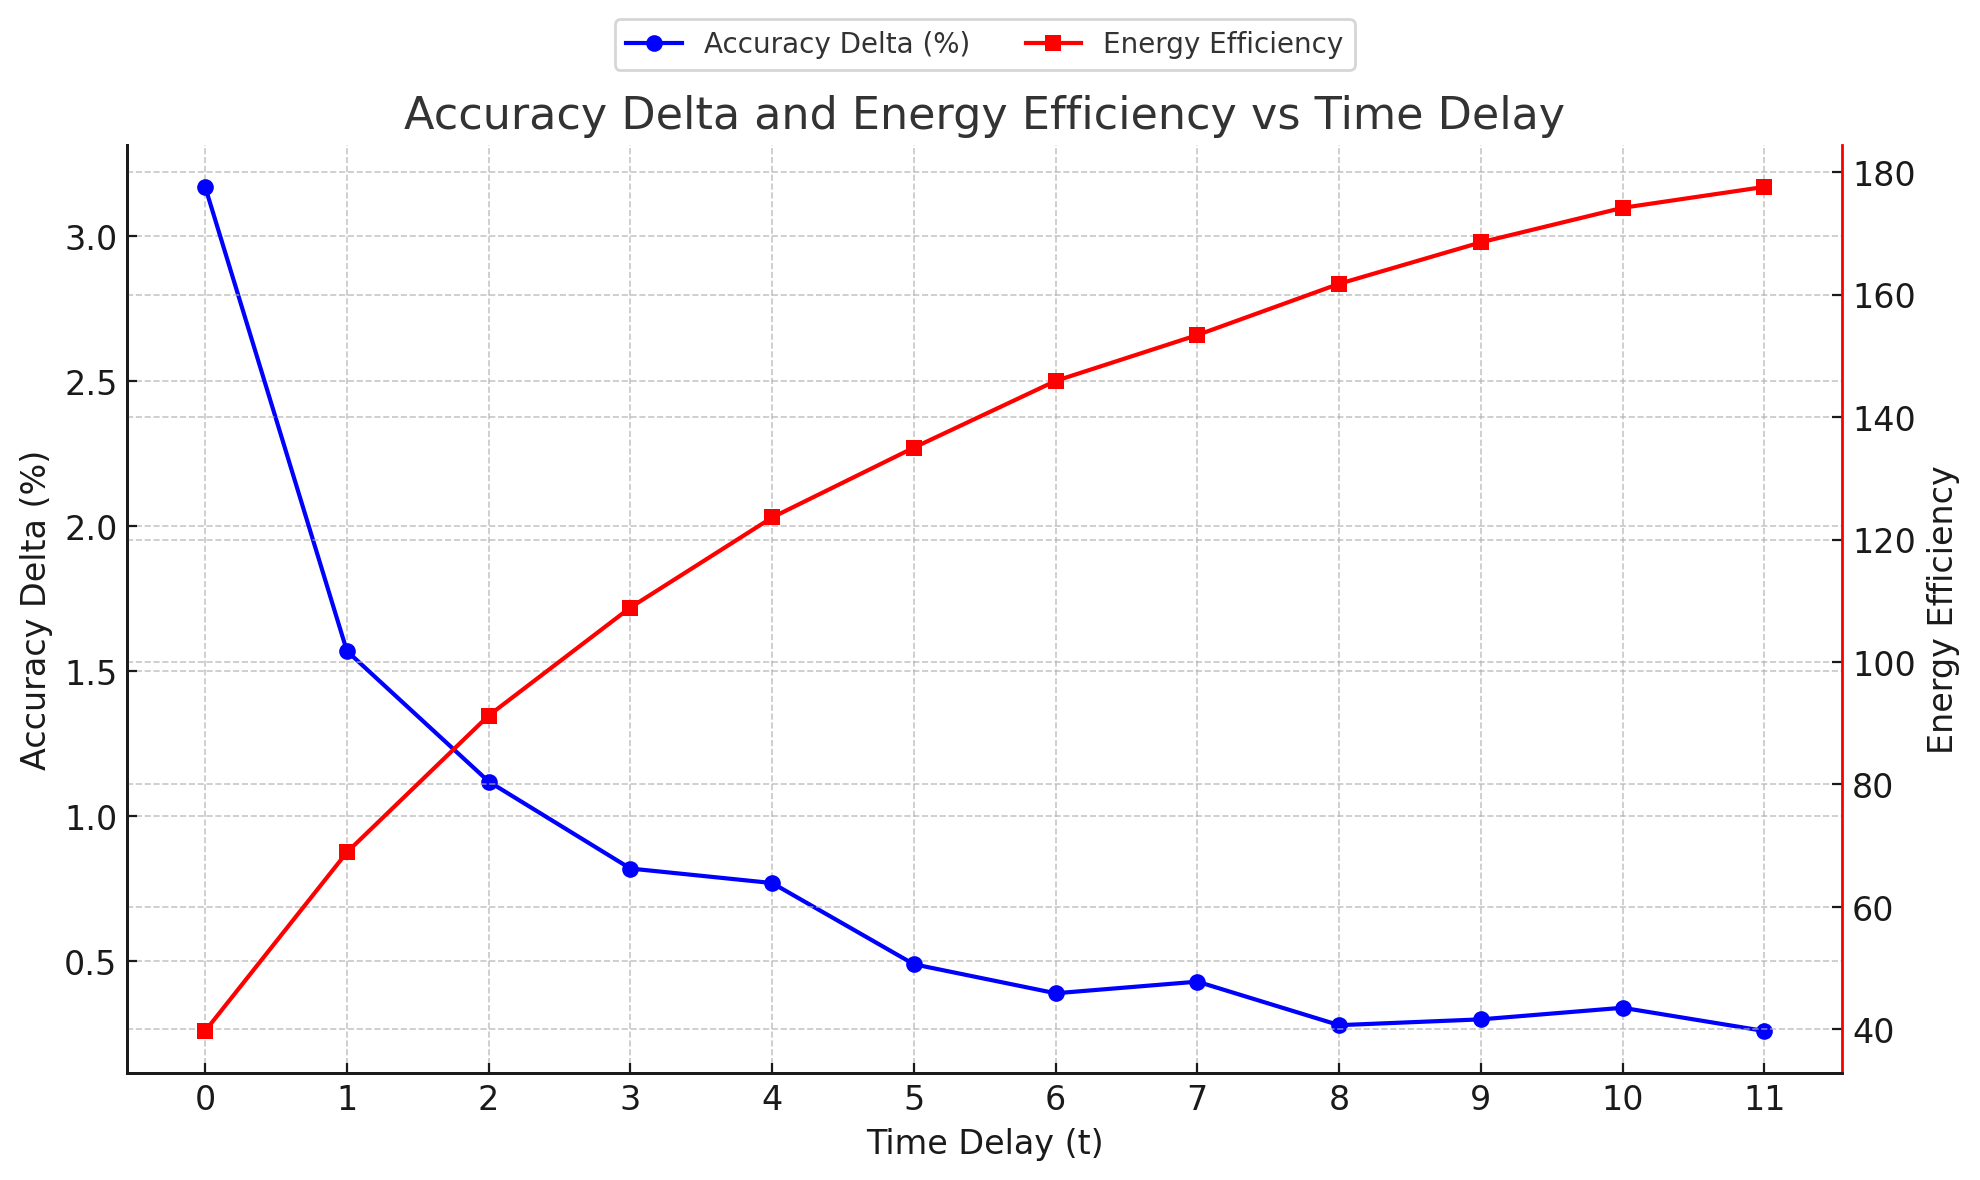
\includegraphics[width=\textwidth]{images/accuracy_tradeoff.png}
  \caption{Accuracy Delta and Energy Efficiency versus Time Delay.  Accuracy Delta represents the performance gain from using the Network Classifier compared to the Edge Classifier alone. Energy Efficiency is inversely proportional to the energy consumed by the communication process.}
  \label{fig:accuracy_tradeoff}
\end{figure}

Conversely, as the Time Delay \(t\) increases, the Network Classifier runs less frequently, drastically reducing the cumulative energy cost. This is reflected in the sharp, monotonic rise of the Energy Efficiency curve, which increases by more than rapidly goes from 0 to 11. This energy saving comes at the cost of accuracy. Since the spatial context is updated less often, its influence diminishes, causing the Accuracy Delta to fall,  and it becomes marginal for \(t > 8\).

This analysis reveals that the system's configuration can be optimized based on deployment needs. For critical applications where maximum accuracy is paramount, a low time delay (\(t=0\) or \(t=1\)) is ideal. However, for long-term monitoring where network longevity is the primary concern, a higher time delay (\(t\ge4\)) can provide substantial energy savings with a modest drop in performance. The region between \(t=1\) and \(t=3\) represents a compelling trade-off where a significant portion of the accuracy gain (1.1\%-1.6\%) is retained while achieving a 2-3 times improvement in energy efficiency over the most aggressive configuration. This demonstrates the flexibility of the HiFiNet architecture, allowing operators to tune the model to strike the right balance between diagnostic accuracy and operational lifetime.


\clearpage
\bibliography{references.bib}
\end{document}
